\documentclass[12pt]{article}
\usepackage[margin=1.25in]{geometry}
\usepackage[final]{microtype}
\usepackage{fontenc}
\usepackage{babel}
\usepackage{float}
\usepackage{graphicx} % images
\usepackage{fancyhdr} % header and footer
\usepackage{algorithm}
\usepackage{algorithmic}
\usepackage{nameref}
\usepackage{cite}
\makeatletter
\newcommand*{\currentname}{\@currentlabelname}
\makeatother

% Page Styling
\pagestyle{fancy}
\lhead{MSE 310 Course Project}
\rhead{\thepage}
\lfoot{Simon Fraser University}
\cfoot{}
\renewcommand{\footrulewidth}{0.4pt}

\title{\textbf{LabView Implementation for an ICT3 Industrial Control Graphical User Interface Controller}}
\author{
  Bansal, Neeraj\\
  \texttt{301xxxxx}
  \and
  Singh, Navjot\\
  \texttt{30xxxxxx}
  \and
  Eshikena, Elvis\\
  \texttt{30132117}
}

\begin{document}
\maketitle

% %%%%%%%%%%%%%%%%%%%%%%%%%%%%%%%%%%%
% Abstract
% %%%%%%%%%%%%%%%%%%%%%%%%%%%%%%%%%%%
\begin{abstract}
The use of automation technology in the world is wide\-spread and a growing field.
Automation is used every\-where from software tasks to machine tasks. The ICT3 platform
is a typical representation of an industrial automation setup. The objective of this
project is to use LabVIEW to develop an efficient and robust, fully automated 
controller for the ICT3 setup to asssemble widgets.

The method used for the base controller was an event prog\-ramming struc\-ture. The
Graphical User Interface GUI was designed for ease of use and learn-time. At
every clock-cycle, all the sensors where scanned for data. When the rigth
sequence of data was read, the corresponding actuator action and program data
were executed and updated respectively.

On an average test cycle, the system was able to reach an accuracy of 100\% on
sorting pegs and rings, 95\% on assembling a ring and peg, 99\% in sensing
which part passes through the Quality Assurance area, and a 100\% in the Rejection
area. The system also is able to save and load a csv file of its outputs using LabViews
file I/O funcatinality. The project demostrated how LabVIEW can be used to program a 
complex controller to automate the ICT3 platform and generate its runtime results.
\end{abstract}
\newpage

% %%%%%%%%%%%%%%%%%%%%%%%%%%%%%%%%%%%
% Table of Contents
% %%%%%%%%%%%%%%%%%%%%%%%%%%%%%%%%%%%
\tableofcontents
\listoffigures
\listoftables
\newpage

% %%%%%%%%%%%%%%%%%%%%%%%%%%%%%%%%%%%
% Introductions
% %%%%%%%%%%%%%%%%%%%%%%%%%%%%%%%%%%%
\section{Introduction}
The ICT3 platform is a representation of a typical industrial automation 
system\cite{ictmanual}. The system includes component sorting, assembly inspection and 
accepts/reject processes. When connected through an interface card or a 
Programmable Logic Controller, the system can
be controlled through a PC.

Using a PC, the sensors and actuators can be programmed to
take-in data through the sensors and manipulate the workspace using the 
actauators.

The objective of the project is to develop an efficient and robust, fully 
automated controller for the ICT setup to asssemble widgets.



% %%%%%%%%%%%%%%%%%%%%%%%%%%%%%%%%%%%
% System Overview
% %%%%%%%%%%%%%%%%%%%%%%%%%%%%%%%%%%%
\section{System Overview}
The system is designed to sort between a metal peg and a plastic ring, assemble
the plastic ring on the metal peg and then determine if the assembly was done 
correctly. It then discards or accepts the item based on the assembly status.

To ensure the system operation and make it easy to use, \textbf{LabView} is used 
to create the FrontPanel GUI alongside the BlockDiagram code.

The sensors and actuators available to us are:
  \begin{itemize}
    \item Actuators
      \begin{itemize}
        \item $FeederActuator$ - Actuator that moves the chain that carries the parts into the system.
        \item $BeltActuator$ - Actuator that moves the belt in second part of the system.
      \end{itemize}
    \item Sorting Area
      \begin{itemize}
        \item $SortSolenoid$ - Solenoid actuator at the sorting area
        \item $SortAreaDetect$ - Infrared sensor which detects when a part is in the area
        \item $SortMetalDetect$ - Inductive sensor which detects if the metal peg is present
        \item $SortSolenoidDetect$ - Inductive sensor which detects the solenoids po\-sition.
      \end{itemize}
    \item Assembly Area
      \begin{itemize}
        \item $AssemblySolenoid$ - This holds rings in a queue to be put into the hopper when it is empty.
        \item $HopperDetect$ - Infrared sensor which tells if a ring is staged in the hopper.
      \end{itemize}
    \item Quality Assurance Area
      \begin{itemize}
        \item $SesningAreaDetect$ - Infrared switch which senses if a part has passed thorugh the QA area
        \item $SensingPegDetect$ - Inductive sensor which detects if a metal peg is present in the QA area.
        \item $SensingRingDetect$ - Capacitive sensor which detects if a plastic ring is ontop of a another part.
      \end{itemize}
  \end{itemize}

\subsection{Graphical User Interface}
  \label{subsec:gui}
  \begin{figure}[H]
    \centering
    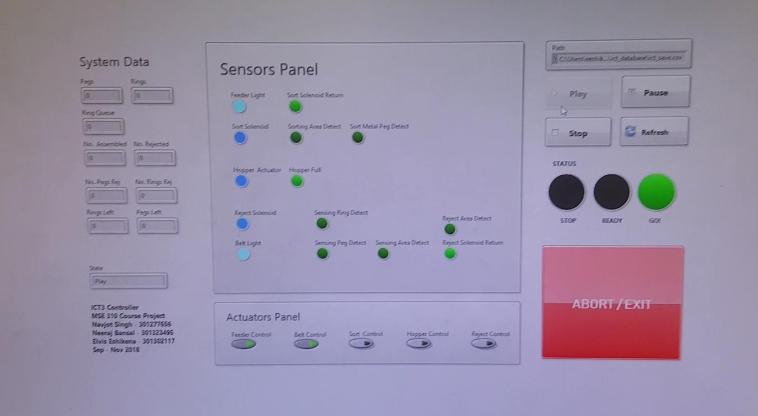
\includegraphics[width=\linewidth]{images/gui.jpg}
    \caption{ICT3 LabView Front Panel}
  \end{figure}

  In making the front panel, the goal was to make it functional, intuitive and beautiful.
  The chosen LabView front-panel framework was the Silver Framework which all the panels
  where made from.

  The positioning of the UI elements were to facilitate spacial similarities to the physical
  ICT3 setup. The panel itself is divided into 3 sections: Controls, Sensors and Actuators, and
  the Output panel. The \textit{Controls} section inlcudes the Play, Pause, Reset and Stop buttons and
  status indicators. The section also contains the Abort/Exit button which helps to exit the program. 
  The \textit{Sensors and Actuators} displayed output LEDs for the status of
  sensors on the ICT3 and toggle switches for the actuators on the ICT3. Finally, the \textit{Outputs}
  panel contained the  values that our system reports back. 
  
  The system reported 9 values of outputs which were:
  \begin{itemize}
    \item $Pegs$ - Number of metal pegs which have entered the system.
    \item $Rings$ - Number of plastic rings which have entered the system.
    \item $RingQueue$ - Number of plastic rings in the hopper queue.
    \item $No.Assembled$ - Number of completed assemblies of ring and peg.
    \item $PegsRej$ - Number of unassembled pegs rejected.
    \item $RingsRej$ - Number of unassembled rings rejeceted.
    \item $TotalRejected$ - Total number of parts rejected.
    \item $PegsLeft$ - Number of pegs left in the system.
    \item $RingsLeft$ - Number of rings left in the system.
  \end{itemize}

  The front panel also includes some \textit{Program Controllers} which are hidden from view.
  These program controllers allow the program save program states and operate on them at another time.
  The \textit{Program Controllers} inlcude:
  \begin{itemize}
    \item $ProgramControl$ - A boolean flag which controls when logic should start to happen.
    \item $ProgramState$ - Controls the state of the state-driven machine which controls the system.
    \item $AssembledFlag$ - A boolean which is true is an assembled piece passed the QA area and false otherwise.
    \item $PegFlag$ - A boolean which is true if only a peg passes the QA area, and false if only a ring
    passes the QA area.
    \item $RejectionControl$ - A number which indicates which action should be taken in the rejection area.
  \end{itemize}

\subsection{Programming}
  The basis of the programming of this LabView virtual instrument was the state-machine method.
  To create the state machine, a case input was modified to create a SubVi of the needed program states.
  The case structure is then placed in an Event Structure which is used to switch states and run the default
  after every 25milliseconds. The event cases then handles all the inputs from software clicks and external
  button presses.

  The program states and their functions are:
  \begin{itemize}
    \item $Init$
      This part of the program controlled the programs variable initializations. It set all the outputs to
      zero, all the booleans to their initial state which are mostly false. It also created the defualt save file
      or loaded the user-directed file. After all these have been setup the program shifts into the $Idle$ case.
    \item $Idle$
      This task is what runs when no process is running in the system. It waits for the play button or the physical
      GO button to be pressed to change its state to the play state. This has the added benefit of having not
      receiving input from anything else if they are mistankenly pressed.
    \item $Play$
      This is the main program state where at every clock pulse actions are taken in the system.
      In this state only the Pause and Stop buttons will be accessible functions. The specific actions
      of the $Play$ state will be explained in the following subsections.
    \item $Pause$
      This state holds the variables of the program and goes into the $Idle$ state.
    \item $Stop$
      This state resets the system and exits the program loop to go start again from the system loop and enter the
      $Init$ state again.
    \item $Abort$
      This state exits the program loop and system loop and also exits the VI.
  \end{itemize}

  The main part of the program is the play state and the following subsection list out the funtions of which the Play
  state does.

  \begin{quote}
    \textbf{\textit{
    The first value which controls everything else is the $Program\-Control$ flag which is set when
    either the $Pegs$ or $Rings$ value is updated once. This signals that all other functions
    should work accordingly because there are parts in the system.}}
  \end{quote}

  \subsubsection{SortingArea.vi}
    \begin{figure}[H]
      \centering
      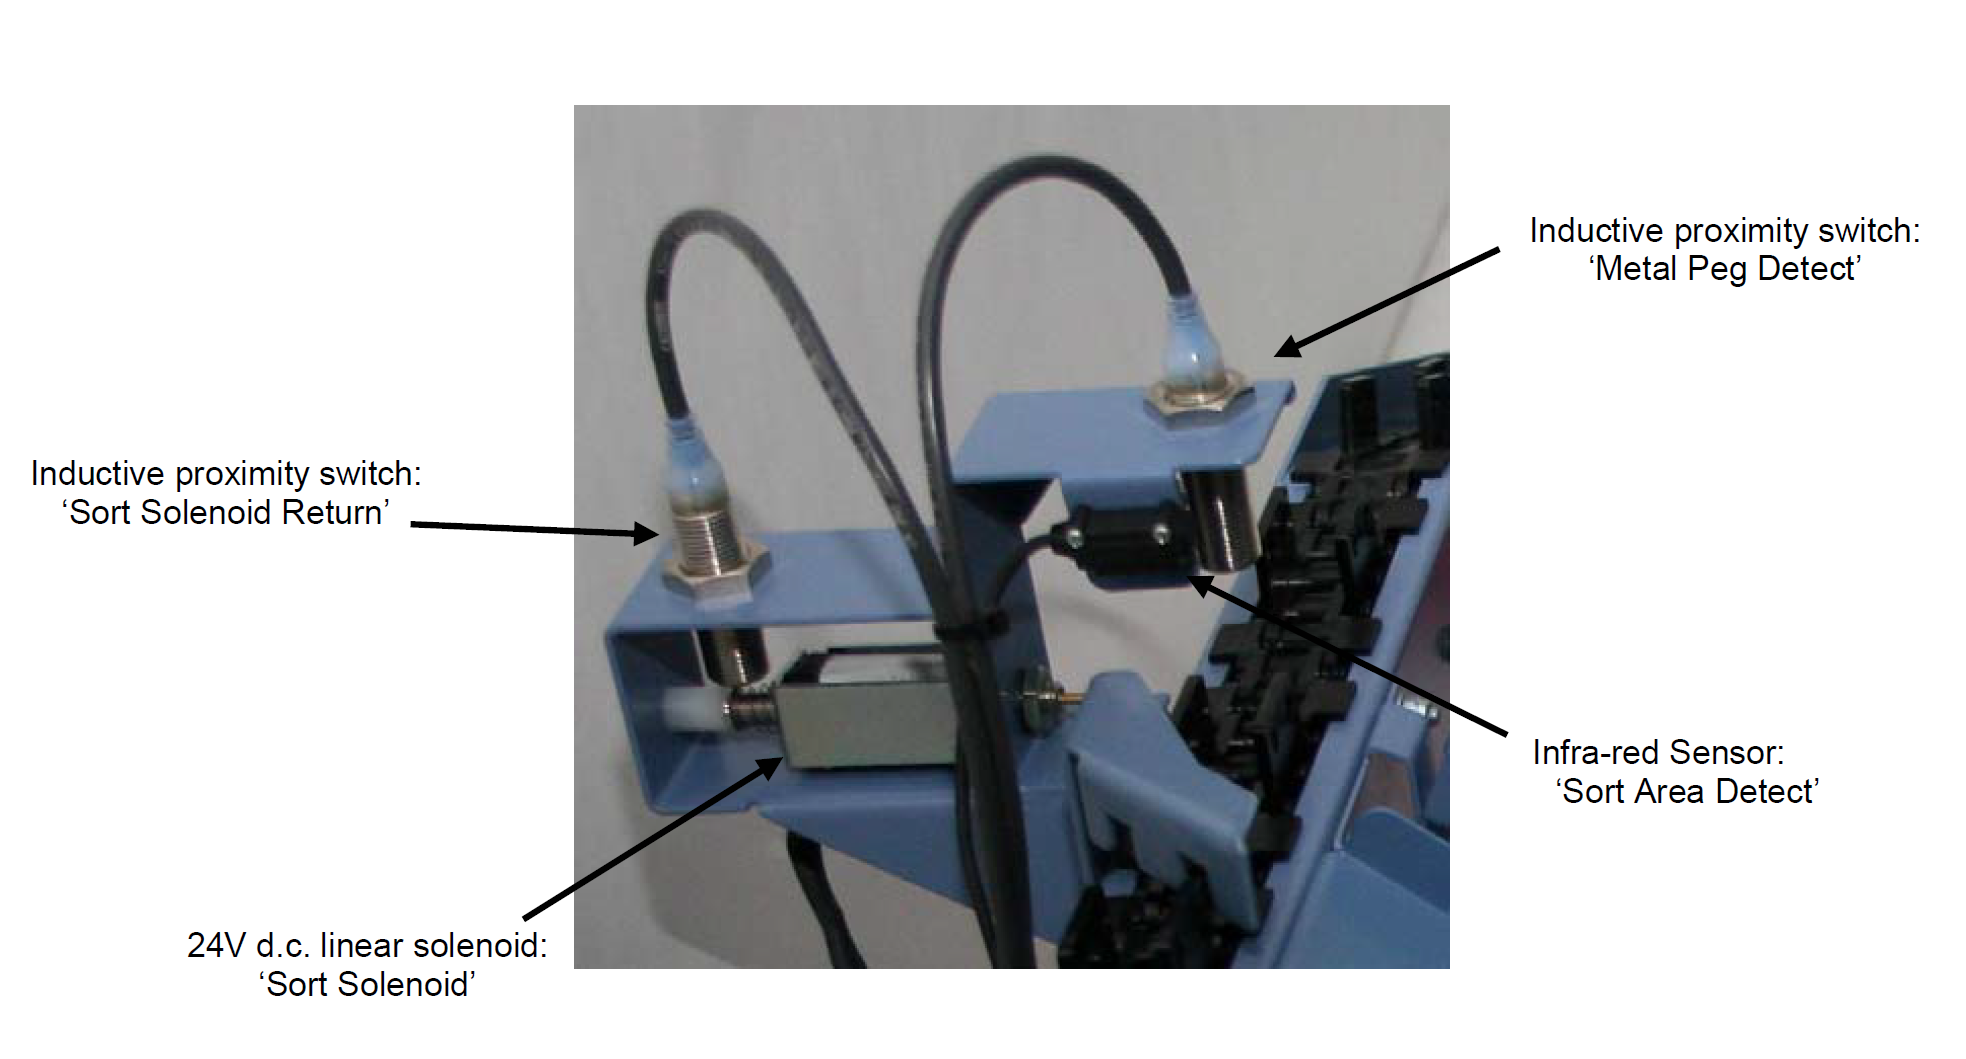
\includegraphics[width=\linewidth]{images/sorting-area.png}
      \caption{Sorting Area\cite{ictmanual}}
    \end{figure}

    At the sorting area, the metal pegs will be sep\-erated
    from the plastic rings. The part will be detected by the $Sort\-Area\-Detect$ 
    sensor. The sensor is position where the part will also be infront of the 
    $SortSolenoid$. If the part is a ring, the solenoid hits it into the 
    assembly chute, if not, it allows it pass down a feeder chute onto the belt
    conveyor. During this process, the $Pegs$ and $Rings$ variables are incremented accordingly.

  \subsubsection{RingQueue.vi}
    A SubVI called \textbf{Ring\-Queue.vi} increments the $Ring\-Queue$ 
    variable when the $Sort\-Solenoid$ is being retracted.

  \subsubsection{AssemblyArea.vi}
    \begin{figure}[H]
      \centering
      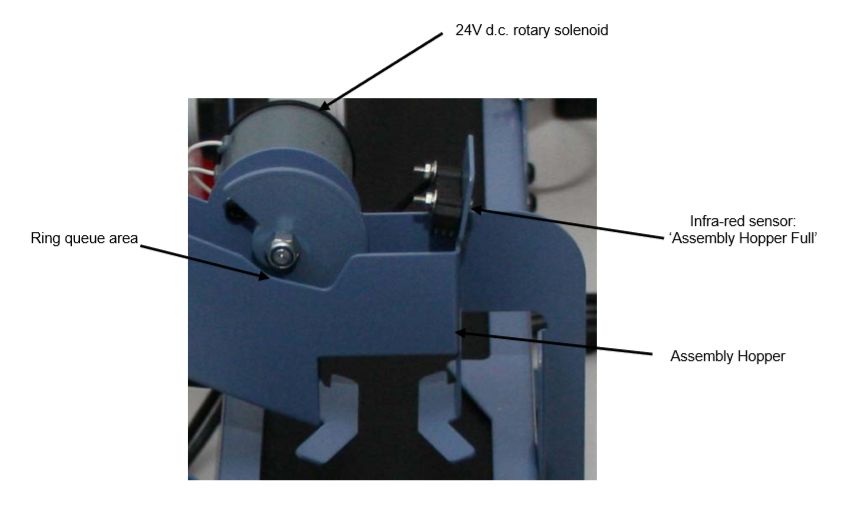
\includegraphics[width=\linewidth]{images/assembly-area.png}
      \caption{Assembly Area\cite{ictmanual}}
    \end{figure}

    When the ring enters the assembly chute, it is staged in a queue by the $Assembly\-Solenoid$.
    When the $RingQueue$ holds 5 rings, further rings are allowed to pass the sorting area.

    The SubVi also checks when the $HopperDetect$ sensor 
    detects that the hopper is empty, the 
    $RotarySolenoid$ allows a ring to be dispensed from the $RingQueue$ into the
    into the hopper and also decrements the $RingQueue$.
    
    When the peg reaches the hopper, it is directed to engage with the hole in the ring
    which makes a complete widget assembly.

  \subsubsection{SensingArea.vi}
    \begin{figure}[H]
      \centering
      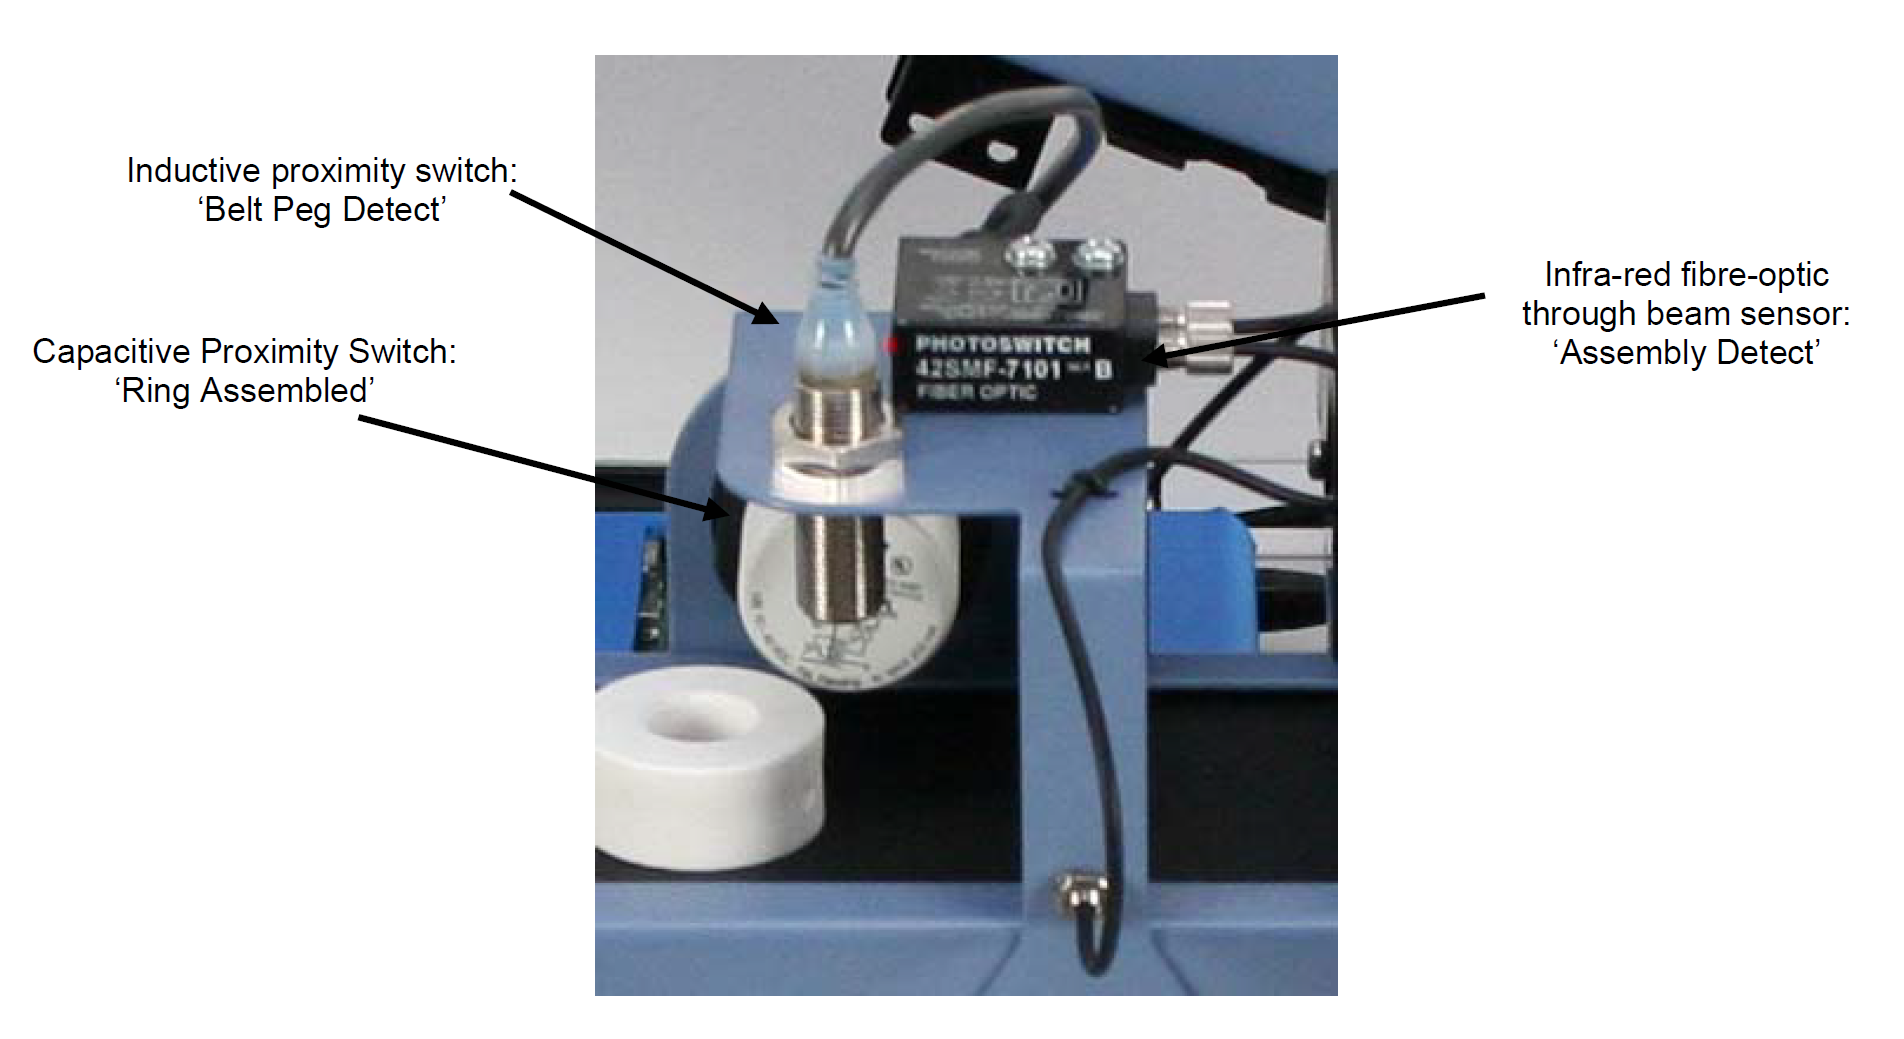
\includegraphics[width=\linewidth]{images/sensing-area.png}
      \caption{Sensing Area\cite{ictmanual}}
    \end{figure}

    At the sensing station, the sesnsors detect if a com\-ponent was ass\-embled or if the
    com\-ponent is a peg or ring. There are three sensors available $Sensing\-Peg\-Detect$, 
    $Sensing\-Area\-Detect$ and the $Sensing\-Ring\-Detect$. 
    Based on the sensors, the $AssembledFlag$ or $PegFlag$ is set or not. which follows the
    following truth table:
    \begin{table}[!ht]
      \centering
      \begin{tabular}{|l|l|l|}
      \hline
      \textbf{AssembledFlag} & \textbf{PegFlag} & \textbf{Output} \\ \hline
      0                      & 0                & Ring            \\ \hline
      0                      & 1                & Peg             \\ \hline
      1                      & x                & Assmebled       \\ \hline
      \end{tabular}
      \caption{Sensing Flags Truth Table}
      \label{tab:flagout}
    \end{table}

    The output from this area is the type of component which is passing the switch. 
    This also sets the $RejectionControl$ program
    controller.

    \begin{table}[!ht]
      \centering
      \begin{tabular}{|l|l|}
      \hline
      \textbf{Output}     & \textbf{RejectionControl} \\ \hline
      Assembled Part      & 1                         \\ \hline
      Single Metal Peg    & 2                         \\ \hline
      Single Plastic Ring & 3                         \\ \hline
      Anything            & 0                         \\ \hline
      \end{tabular}
      \caption{Rejction Control Lookup Table}
      \label{tab:rejout}
    \end{table}

  \subsubsection{RejectionArea.vi}
    \begin{figure}[H]
      \centering
      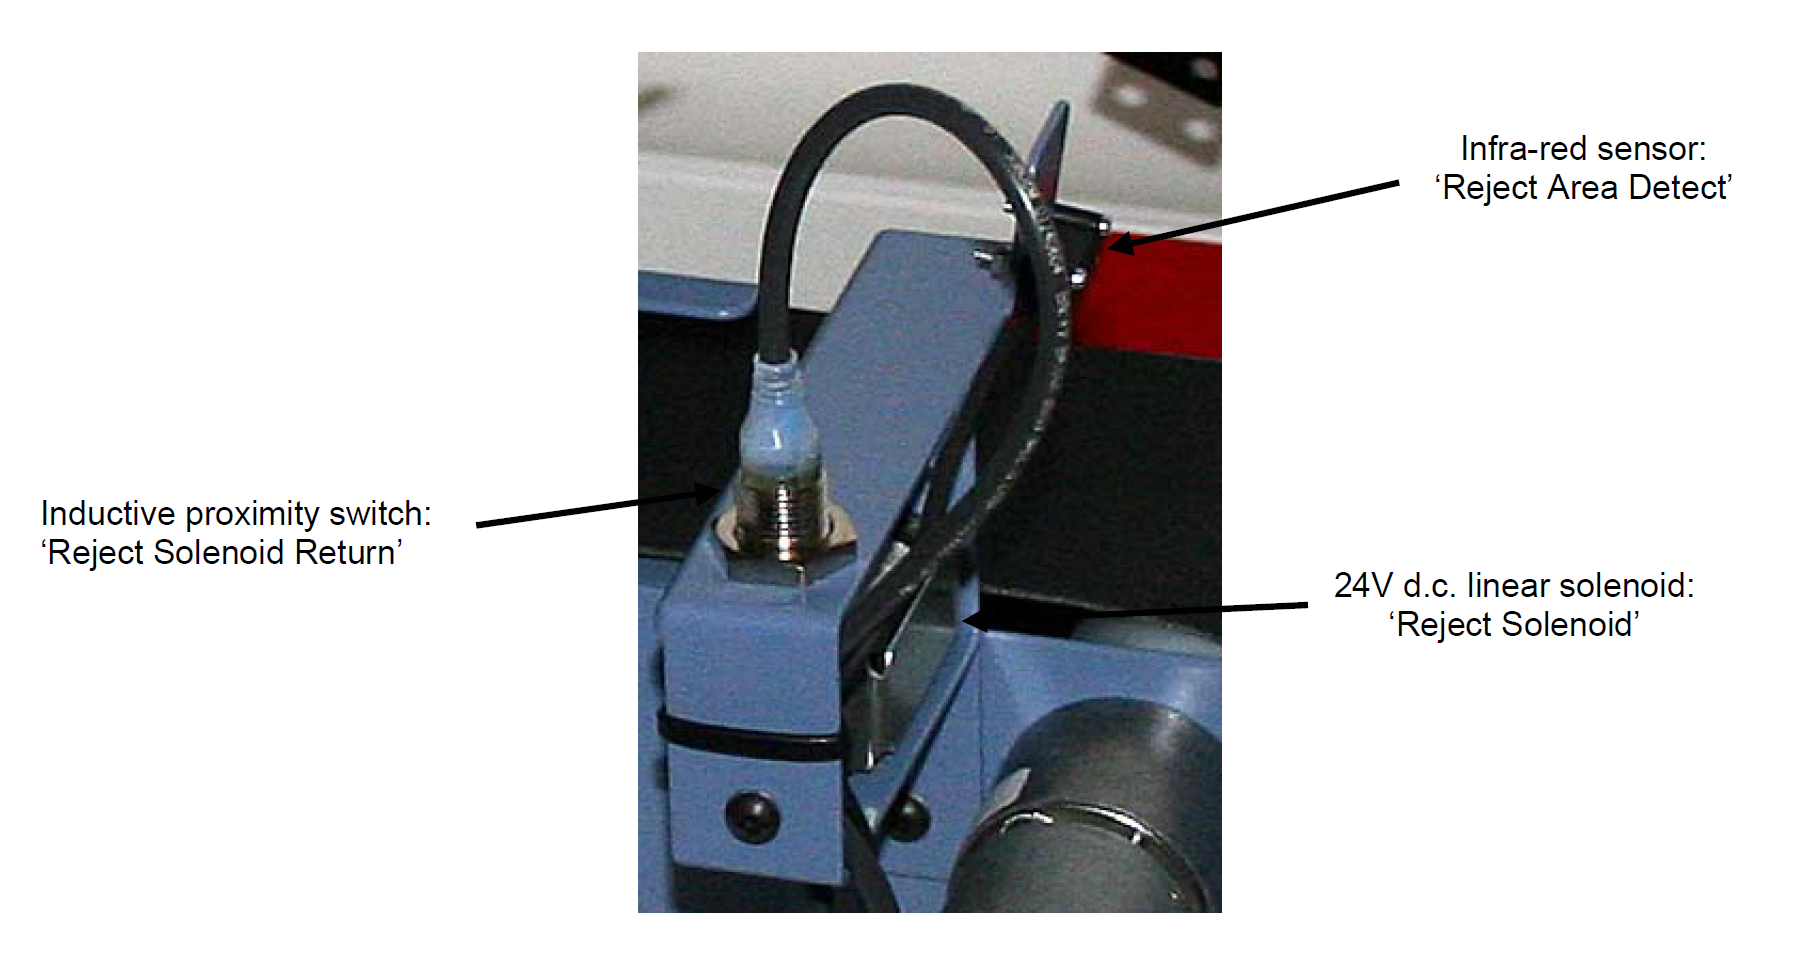
\includegraphics[width=\linewidth]{images/reject-area.png}
      \caption{Rejection Area\cite{ictmanual}}
    \end{figure}

    When the component from the sensing station is detected by the $Reject\-Area\-Detect$
    sensor, it uses the data from the $RejectionControl$ to act on the component. 
    If it is either a single ring or peg, the $RejectSolenoid$ is activated else, it allows an
    assembled part to pass through.

    Afterwards it resets the $AssembledFlag$, $PegFlag$ and $RejectionControl$ to false and 0
    respectively.


% %%%%%%%%%%%%%%%%%%%%%%%%%%%%%%%%%%%
% Algorithms
% %%%%%%%%%%%%%%%%%%%%%%%%%%%%%%%%%%%
\section{Algorithms}
This section highlights the logic if the different sections of the system.
A list of program variables which will be tracked and referenced can be found in 
Section \ref{subsec:gui}

\subsection{The Sorting Area}
  The sorting area algorithm differentiates between a ring and a peg by reading the edges of the
  $SortMetalDetect$ and $SortAreaDetect$ signals.

  If the area sensor is rising then something is detected, if the metal sensor is then falling,
  the part is most definitely a metal peg else it is treated as a plastic ring and put into the
  assembly queue.

  \begin{algorithm}[H]
    \caption{\currentname}
    \begin{algorithmic}
      \REQUIRE $t$ - time count
      \STATE $A \Leftarrow SortAreaDetect$
      \STATE $M \Leftarrow MetalPegDetect$
      \STATE $S \Leftarrow SortSolenoidReturn$
      \WHILE {$ProgramControl = 1$}
        \IF{$[t]=1\,and\,A[t-1]=0$}
          \IF{$M[t]=M[t-1]$}
          \STATE $SortSolenoid \leftarrow 1$
          \STATE $Rings \leftarrow Rings + 1$
          \ELSE
            \STATE $Pegs \leftarrow Pegs + 1$
          \ENDIF
        \ENDIF

        \IF{$S[t]=1 \land S[t-1]=0$}
          \STATE $RingQueue \leftarrow RingQueue + 1$
        \ENDIF
      \ENDWHILE
    \end{algorithmic}
  \end{algorithm}

\subsection{The Assembly Area}
  In the asssembly area, if the $AssemblyAreaDetect$ detects that its empty and there is a ring a available 
  in the $RingQueue$ then the solenoid opens for $\frac{1}{2}$ a second. If the RingQueue was previously
  empty, then wait for $\frac{1}{2}$ a second before opening it. Afterwards, decrease the $RingQueue$.

  \begin{algorithm}[H]
    \caption{\currentname}
    \begin{algorithmic}
      \REQUIRE $t$, The time count
      \WHILE {$ProgramControl = 1$}
        \IF {$AssemblyAreaDetect = False \land (RingQueue \geq 1)$} 
          \IF {$RingQueue[t-1] = 0$}
            \STATE Wait for $500ms$
          \ENDIF
          \STATE $RotarySolenoid \leftarrow 1$
          \STATE Wait for $500ms$
          \STATE $RingQueue \leftarrow RingQueue - 1$
        \ELSE
          \STATE $RotarySolenoid \leftarrow 0$
        \ENDIF
      \ENDWHILE
    \end{algorithmic}
  \end{algorithm}

\subsection{The Sensing Station}
  At the sensing station, if the $SensingPegDetect$ is activated the $Pegflag$ should be set. 
  If the $SensingRingDetect$ is activated then the $AssembledFlag$ should be set.
  If the $SensingAreaDetect$ is on it s rising signal edge, both flags are checked and the
  outputs to the $RejectionControl$ are decided based on Table \ref{tab:flagout} and
  Table \ref{tab:rejout}.

  \begin{algorithm}[H]
    \caption{\currentname}
    \begin{algorithmic}
      \REQUIRE $t$, The time count
      \STATE $A \Leftarrow SensingAreaDetect$
      \STATE $P \Leftarrow BeltPegDetect$
      \WHILE {$ProgramControl = 1$}
        \IF {$RingAssembledDetect$}
          \STATE $AssembledFlag \leftarrow 1$
        \ENDIF

        \IF {$BeltPegDetect$}
          \STATE $PegFlag \leftarrow 1$
        \ENDIF

        \IF {$A[t]=1 \land A[t-1]=0$}
          \IF {$AssembledFlag=1$}
            \STATE $RejectionControl \leftarrow 1$
            \STATE $AssembledFlag \leftarrow 0$
          \ELSE [AssembledFlag not set]
            \IF {$PegFlag=1$}
              \STATE $RejectionControl \leftarrow 2$
              \STATE $PegFlag \leftarrow 0$
            \ELSE [PegFlag not set]
              \STATE $RejectionControl \leftarrow 3$              
            \ENDIF
          \ENDIF
        \ENDIF
      \ENDWHILE        
    \end{algorithmic}
  \end{algorithm}

\subsection{The Reject Area}
  At the rejection area, if the $RejectAreaDetect$ is on its rising edge,
  the value assinged in the $RejectionControl$ variable is checked and based on that,
  single pegs and rings are ejected by setting the $RejectionControl$ to true and the assembled
  parts are allowed to pass through by setting the opposite-false value.

  Afterwards, when the $RejectSolenoidReturn$ is on its signal rising edge, the total Number
  of rejected parts are recalculated.

  \begin{algorithm}[H]
    \caption{\currentname}
    \begin{algorithmic}
      \REQUIRE $t$, The time count
      \STATE $A \Leftarrow RejectAreaDetect$
      \STATE $R \Leftarrow RejectSolenoidReturn$
      \WHILE {$ProgramControl = 1$}
        \IF {$A[t]=1 \land A[t-1]=0$}
          \IF {$RejectionControl=1$}
            \STATE $RejectSolenoid \leftarrow 0$
            \STATE $No.Assembled \leftarrow No.Assembled + 1$
          \ELSIF {$RejectionControl=2$}
            \STATE $RejectSolenoid \leftarrow 1$
            \STATE $PegsRej \leftarrow PegsRej + 1$
          \ELSIF {$RejectionControl=3$}
            \STATE $RejectSolenoid \leftarrow 1$
            \STATE $RingsRej \leftarrow RingsRej + 1$
          \ELSE [No predefined state]
            \STATE Do nothing
          \ENDIF
          \STATE $RejectionControl \leftarrow 0$
        \ENDIF
      \ENDWHILE
    \end{algorithmic}

    \begin{algorithmic}
      \REQUIRE $t$ - loop variable counter
      \STATE $R \leftarrow RejectSolenoidReturn$
      \IF {$R[t] = 1 \land R[t-1]=0$}
        \STATE $TotalRejected \leftarrow RingsRej + PegsRej$
      \ENDIF
    \end{algorithmic}
  \end{algorithm}

\subsection{Program execution}
  The program execution algorithm highlights the calculations that happen in every loop.
  This is where the $PegsLeft$ and $RingsLeft$ are calculated. and the saving of output data
  occurs every 20 seconds.

  $PegsLeft$ and $RingsLeft$ are calculated by subtracting the number of assembled pieces and the
  number of rejected pieces from the number that entered the system.

  \begin{algorithm}[H]
    \caption{\currentname}
    \begin{algorithmic}
      \WHILE {$ProgramControl = 1$}
        \STATE $PegsLeft \leftarrow Pegs - No.Assembled - PegsRej$
        \STATE $RingsLeft \leftarrow Rings - No.Assembled - RingsRej$
      \ENDWHILE
    \end{algorithmic}
  \end{algorithm}


% %%%%%%%%%%%%%%%%%%%%%%%%%%%%%%%%%%%
% Discussions
% %%%%%%%%%%%%%%%%%%%%%%%%%%%%%%%%%%%
\section{Discussion}
The study of the development of a LabView GUI for the ICT3 platform has the relevance of learning
how to program visually and implementing control systems for industial automation. The ICT3 provides
practice on logical thinking and developing robust algorithms to handle different cases in properly.
During the development of the system, inspiration was taken from concepts in \textbf{Digital Logic}
such as gate-level reduction and edge-triggered events. Samples of where these were utilized are:
In the Sensing area, only one sensor is used to determine an assembled peice and at
the Sorting Area, a metal piece is recognized on the falling edge of the the metal detect sensor.

Being an educational tool used thorughout the year, 
the system is not without its limitations and being a mechanical system,
it is prone to mechanical error. For example, in the Sorting Area, when the solenoid pushes a Ring
part, experiment has shown that it can get stuck in the shute before it is staged at the 
Assembly Solenoid. This error reflects on the system computations and if occur can be corrected by
manual correction.

Another mechanical error which can occur is when the Assembly Solenoid opens, the ring part can get
staged wrongly and stage horizontally instead of vertically. This error can be corrected by manually
lifting the staged part. To facilitate manual correction the system can easily be paused and corrected.

The most challenging protion of the system development was the assembly chute area. Every other part
of the system had semi-realtime processing. That is, when anything was sensed, action would be taken
in the same instant. In the section between the Assembly chute area, the logic needed to
be delayed to make sure the AssemblySolenoid does not open and close randomly.
To meet this requirement, 2 alternate algorithms were developed, one which was able to assemble 
rings and pegs without error but with lots of rejected pegs (depending on the input order), and another
which was able to assemble most rings and pegs but with some margin of error.

The less accurate algorithm worked by only opening the Assembly Solenoid when there is nothing in the
Hopper, there is a ring or more in the Ring Queue and a peg is detected at the Sorting Station. 
This method was not used because when multiple 
metal pegs pass thorugh, the time between consecutive incoming pegs, does not match the time it takes
for the first peg to clear the ring in the Hopper. While the second algorithm, the one which was used
opens the Assembly Solenoid when the Hopper is empty and there was a ring in the Ring Queue. The major
difference being, it was opened for a fixed amount of time - 0.5 seconds. To combat the initial mechanical
error discussed, when there was no Ring in the Queue, there was delay to make sure the part had reached
the bottom of the Assembly chute on average.

If time allows, further reearch into how the input feeder chain affects the timing of the system and how
to minimize algorithms to make them use less variables but more focus on processing the signals coming
from the sensors.

% %%%%%%%%%%%%%%%%%%%%%%%%%%%%%%%%%%%
% Conclusions
% %%%%%%%%%%%%%%%%%%%%%%%%%%%%%%%%%%%
\section{Conclusions}
The objective of this project was to design a GUI controller for the ICT3 system using LabViews Graphical
programming language. The importance of this project stems from its positoin as a building block to
industrial automation and control systems. It serves as a practical application of Sensors and actuators
knowledge and using concepts from other engineering fields, robust controllers can be built to achieve
repeateable tasks.

The controller implementation in this repot used concepts from digital logic and apllied different 
strategies in tackling the goals in each section. Sorting, in the sorting area was achieved by actions 
based on edge-trigerring, Assembly in the assembly chute and hopper was based on timing, Sensing
was based on edge-triggering and state flags and finally, Rejection was solely based on flags.

From these implementations,the system was able to reach an accuracy of 100\% on
sorting pegs and rings, 95\% on assembling a ring and peg, 99\% in sensing
which part passes through the Quality Assurance area, and a 100\% in the Rejection
area. The system also is able to save and load a csv file of its outputs using LabViews
file I/O funcatinality.

When developing these solutions the areas were examined seperatedly and not as a whole. This whole view,
may offer some more insight into more optimisations for the system and has been offered has a topic that
warrants futher research. The project demostrated how LabVIEW can be used to program a 
complex controller to automate the ICT3 platform and generate its runtime results and these coding structure
can be applied to any realtime desktop controller system.

\clearpage
\bibliographystyle{IEEEtran}
\bibliography{MSE310_ProjectReport}
\end{document}
